\documentclass{ximera}

\newcommand{\RR}{\mathbb R}
\renewcommand{\d}{\,d}
\newcommand{\dd}[2][]{\frac{d #1}{d #2}}
\renewcommand{\l}{\ell}
\newcommand{\ddx}{\frac{d}{dx}}
\newcommand{\dfn}{\textbf}
\newcommand{\eval}[1]{\bigg[ #1 \bigg]}


\author{Jason Miller}
\license{Creative Commons 3.0 By-NC}


\outcome{}


\begin{document}
\begin{exercise}
Use trig substitution to determine the integral.
\[
\int \frac{1}{(1+x^{2})^{2}} \d x
\]

First we must determine the appropriate substitution. 

Since we have a $1+x^{2}$ term, we should use $x=\answer{\tan(\theta)}$. 

This means that $\d x= \answer{ \sec^{2}(\theta)} \d \theta$. 

\begin{exercise}
Using the trig identity $1+\tan^{2}(\theta)=\sec^{2}(\theta)$, we can rewrite $1+x^{2}$ as $\answer{\sec^{2}(\theta)}$. 

Now we can express our original integral as a trigonometric integral in terms of the variable $\theta$. 

\[
\int \frac{1}{(1+x^{2})^{2}} \d x= \int \answer{ \cos^{2}(\theta)} \d \theta\
\]

The antiderivative in terms of $\theta$ is 

\[
\answer{ \frac{1}{2}\theta + \frac{1}{2}\sin(\theta)\cos(\theta) + C}
\]
(Use $C$ for the constant of integration)

\begin{hint}
The following trig identities will be useful.
\begin{align}
\cos^{2}(\theta)&=\frac{1+\cos(2\theta)}{2} \\
\sin(2\theta)&=2\sin(\theta)\cos(\theta)
\end{align}
\end{hint}

Now we really want the antiderivate in terms of $x$ since our functions was originally in terms of $x$. 

\begin{exercise}
Using the original substitution $x=\tan(\theta)$, we draw the right triangle 

    \begin{image}
      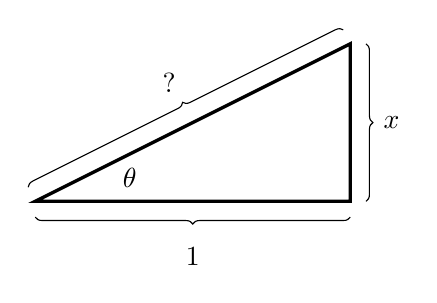
\begin{tikzpicture}
        \coordinate (C) at (0,2);
        \coordinate (D) at (4,2);
        \coordinate (E) at (4,4);
        \tkzMarkRightAngle(C,D,E)
        \tkzMarkAngle(D,C,E)
        \draw[decoration={brace,mirror,raise=.2cm},decorate,thin] (0,2)--(4,2);
        \draw[decoration={brace,mirror,raise=.2cm},decorate,thin] (4,2)--(4,4);
        \draw[decoration={brace,raise=.2cm},decorate,thin] (0,2)--(4,4);
        \draw[very thick] (D)--(E)--(C)--cycle;
        \node at (2,2-.7) {$1$}; %% adj
        \node[anchor=west] at (4+.3,3) {$x$}; %% opp 
        \node at (2-.3,3+.5) {$?$}; %% hyp
        \node at (1.2,2.3) {$\theta$};
      \end{tikzpicture}
    \end{image}

Then using the Pythagorean Theorem we find that the
 length of the hypotenuse=$\answer{\sqrt{1+x^{2}}}$. 

Using the triangle, we now convert each of the expressions in our antiderivative that was in terms of $\theta$ to be in terms of $x$:

\begin{align}
\theta&=\answer{\arctan(x)} \\
\sin(\theta)&=\answer{\frac{x}{\sqrt{1+x^{2}}}} \\
 \cos(\theta)&=\answer{\frac{1}{\sqrt{1+x^{2}}}} 
\end{align}

\begin{exercise}
Hence the answer to our original integral is: 

\[
\int \frac{1}{ (1+x^{2})^{2}} \d x= \answer{ \frac{1}{2}\arctan(x) + \frac{x}{2(1+x^{2})} + C }
\]
(Use $C$ for the constant of integration)





\end{exercise}
\end{exercise}

\end{exercise}

\end{exercise}
\end{document}
